\documentclass[12pt]{report}

\usepackage{blindtext}
\usepackage{listings,xcolor}
%\usepackage[T1]{fontenc}
\usepackage[francais]{babel}
\usepackage[utf8]{inputenc}
%\usepackage[pdftex]{graphicx}
%\usepackage{xcolor}
\usepackage{enumitem}
%\usepackage{listings}
\usepackage{graphicx}
%\usepackage[export]{adjustbox}
%\usepackage{wrapfig}
\usepackage{titlesec}
\usepackage{hyperref}
%\usepackage{ulem}

\usepackage[a4paper,left=2cm,right=2cm,top=2cm,bottom=2cm]{geometry}
\usepackage{libertine}

\setlength{\parindent}{0cm}
\setlength{\parskip}{1ex plus 0.5ex minus 0.2ex}
%\newcommand{\hsp}{\hspace{20pt}}
\newcommand{\HRule}{\rule{\linewidth}{0.5mm}}
\titleformat{\chapter}[display]
  {\normalfont\bfseries}{}{0pt}{\Large}

\begin{document}

\begin{titlepage}
  \begin{sffamily}
  \begin{center}
    \begin{minipage}{1\textwidth}
    \end{minipage}
    \newline
    \newline
    \newline
    \newline
    \newline
    \newline
    \newline
    \newline
    \newline
    \newline
    \newline
    \textsc{\LARGE Université de Valenciennes et du Hainaut-Cambrésis}\\[4cm]
    \HRule \\[0.4cm]
    { \huge \bfseries M2C - Malware Clustering et Classification\\[0.4cm] }
    \HRule \\[2cm]
    \begin{figure}[htpb]
    \center
	
\includegraphics[width=13cm,height=6.5cm]{img/datascience.png}
    \end{figure}
     \center
        Vincent \textsc{Romé} -
        Axel \textsc{Foulon} -
        Julien \textsc{Dupagny}
         \center
       	{vrome/afoulon/jdupagny}@etu.univ-valenciennes.fr

    \vfill
    {\large — 9 Juin 2018 —}
  \end{center}
  \end{sffamily}
\end{titlepage}
\newpage
\begin{center}
\begin{tabular}{|l|c|l|c|}
   \hline
   \multicolumn{4}{|c|}{HISTORIQUE DES VERSIONS} \\
   \hline
   DATE & VERSION & ÉVOLUTION DU DOCUMENT & RÉDACTEUR \\
   \hline
   9/06/2018 & 0.1 & Version préliminaire & Équipe complète \\
   \hline
\end{tabular}
\end{center}
\tableofcontents

\chapter{Notice légale}
	Le présent document présente et exprime, sauf indication contraire, le fruit de la recherche de la réflexion, des idées et du développement d’une solution pouvant répondre aux besoins et aux spécifications du marché de la cyber sécurité en matière de détection de malware. Ce document doit être considéré dès lors comme les points de vue et interprétation des auteurs. Ce document ne reflète pas nécessairement l’état de la technologie la plus récente et pourrait faire l’objet de mises à jour.
\newline\newline
	Les sources tierces seront citées, le cas échéant, l’équipe du projet acceptera d’étudier toute requête en cas d’oubli cependant elle ne reste pas responsable du contenu des sources extérieures.
Le dit document a une vocation strictement informative. Toute personne possédant un exemplaire de ce document pourra être tenu responsable de l’usage qu’il pourrait en faire.
\newline\newline
Tous droits réservés. Ce document doit dès lors être considéré comme propriété intellectuelle (cf Code de la propriété intellectuelle / loi 92-597) des auteurs de ce dernier à savoir Vincent ROME et Axel FOULON et Julien DUPAGNY. Aucune partie de cette publication ne peut être reproduite ou partiellement reproduite, stockée dans un système de recherche documentaire ou transmise sous quelque forme ou par quelque moyen que ce soit - électronique, mécanique, photocopie, enregistrement ou autre - sans l’accord préalable écrit par l’ensemble des membres de l’équipe, sauf dans la mesure expressément autorisée par la loi ou aux conditions convenues avec les organismes compétents en matière de droits. Dans tous les cas, la mention de la source est obligatoire. Tout non respect et ou diffusion de ce présent de ce document pourra engendrer des poursuites prévues par la loi.

\chapter{Introduction}
	Jusqu'à présent les systèmes de détection d'intrusion reposaient traditionnellement sur des signatures générées manuellement par des experts en sécurité, puis nous avons vu apparaître des systèmes permettant de détecter des patterns entre des jeux de données ceci a permis de générer automatiquement ces règles. Aujourd’hui avec l’apparition du “Big Data” des solutions comme le Deep Learning ou  Machine learning sont souvent présentés comme les technologies pouvant révolutionner les systèmes de détections et les performances.
Ces systèmes permettent de générer automatique un modèle de détection à partir de données et leurs capacités à généraliser les événements malveillants permettait en effet de détecter des éléments encore inconnus.
\newline\newline
	L’objectif est d’ici comprendre le fonctionnement de ces algorithmes et de les appliquer au milieu de la sécurité informatique. D’exposer les résultats de notre recherche sur la détection de fichier PE (exécutable windows malveillants). Tout en gardant un regard critique sur les résultats et en essayant d’apporter des solutions sur l’utilisation de tel algorithme en production.
\newline\newline
	Un modèle de détection supervisée est construit à partir de données labellisées fournies par l’expert : des événements bénins, mais aussi des événements malveillants pour guider le modèle de détection. L’algorithme d’apprentissage va automatiquement chercher les points permettant de caractériser chacune des classes ou de les discriminer pour construire le modèle de détection.

\chapter{Abstract}
	Until now, intrusion detection systems have traditionally relied on signatures generated manually by security experts, and we have seen systems for detecting patterns between datasets that have automatically generated these rules. Today with the emergence of "Big Data" solutions such as Deep Learning or Machine Learning are often presented as technologies that can revolutionize detection systems and performance.
These systems make it possible to automatically generate a detection model from data and their ability to generalize malicious events made it possible to detect unknown elements.
\newline\newline
	The goal here is to understand how these algorithms work and apply them to the computer security environment. To expose the results of our research on PE file detection (executable malicious windows). While keeping a critical eye on the results and trying to provide solutions on the use of such algorithm in production.
\newline\newline
	A supervised detection model is built from labeled data provided by the expert: benign events, but also malicious events to guide the detection model. The learning algorithm will automatically look for the points to characterize each of the classes or to discriminate them to build the detection model.

\chapter{Contexte du projet}
Le master CDSI (Cyber-defense, sécuritée de l’information) est une formation qui à pour objectif de fournir les competences scientiques aux concepts, méthodes et techniques de traitement de la securité et de la gestion du risque liées aux systèmes d’information et sachant protéger les ressources d’un systeme d’information. Cette formation peut être éffectuée en formation initiale ou en formation continue. Elle depend de l’Institut des Sciences et Techniques de Valenciennes. 
Ce document constitue le memoire d'un projet  universitaire ayant  été dans le cadre  de ce master en formation universitaire sur le campus de Maubeuge.
	Dans le cadre du module "Programmation distribuée et sécurité/ Sécurité des systèmes embarquée" nous avons eu l'occasion de réaliser un travail pratique sur le ML (Machine Learning).

\chapter{Les contraintes}
Il est dès à présent nécessaire de prendre en compte plusieurs contraintes que nous ne ne devons pas perdre de vu:
\begin{itemize}[label=\textbullet]
	\item Prédiction rapide
	\item Mise à jour périodique du modèle
	\item Interprétable (Expert puisse comprendre le modèle et l’ajuster)
\end{itemize}

\chapter{Les objectifs}
A travers ce projet nous voulons fournir une solution permettant la classification et une détection via des algorithmes de machine learning de malwares touchant les systèmes d’exploitation Windows de Microsoft.
\newline\newline
Nous pourrons découvrir le principe de base d’une analyse statique de fichier malveillant, ainsi que les notions relatives au machine learning et la data science pour le traitement de gros flux de données. Il s'agit d'une application particulière en matière de sécurité informatique des nouveaux algorithmes qui ont le vent en poupe.
\newline\newline
L'objectif est qu'à l'issue de ce projet, nous soyons en mesure de comprendre les notions de base relative à :
\begin{itemize}[label=\textbullet]
	\item L'analyse de malwares
	\item Les algorithmes d'apprentissage automatique
	\item Comprendre le workflow associé à l'utilisation de tels algorithmes.
\end{itemize}
A l'issue de ce projet un PoC d'implémentation en python devra être disponible.
Des premiers résultats permettront de conclure sur l'efficacité et la complexité ainsi que les limitions de tels algorithmes appliqué dans le domaine de la sécurité.
\part{Généralités}
\chapter{Les formes d’analyses de malware}
\section{Analyse statique}
L’analyse statique peut être vu comme le fait de “lire” le fichier malware sans l'exécuter afin d’essayer d’émettre des hypothèses sur son fonctionnement à partir de ces propriétés.
Il existe plusieur technique qui peuvent être utilisé afin d’effectuer ce type d’analyse.


Voici des exemples :
\begin{enumerate}
	\item L’analyse du format du fichier ( Parsing): La structure du fichier est standardisé, elle nous permet d’en extraire des métadonnées qui peuvent être utiles. Par exemple : (les fichiers importés, la date de compilation…)
	\item L’extraction de chaîne de caractères
	\item Dissasembly: Cette technique consiste aux reverse engineering des instructions assembleurs du programme afin de comprendre la logique interne du programme.
\end{enumerate}

Cette technique de détection à donc pour objectif de classifier les échantillons sans les exécuter, Elle possède l’avantage d’être une couche de protection lorsque la détection fonctionne car elle permet de détecter des fichiers malveillant avant qu’il ne soit exécuté.

	
\section{Analyse Dynamique}

\chapter{Malware Taxonomy}

Pour avoir une meilleure compréhension des méthodes et de la logique derrière les logiciels malveillant dit malware. Nous pouvons les classer selon l’objectif visé par le pirate. Les grandes classes sont les suivantes:
\begin{enumerate}
	\item Les Virus
	\item Les Vers - Worm
	\item Les Chevaux de Troy - Trojan
	\item Les portes dérobées - Backdoor
	\item Les Rootkit
	\item Les robots - Bot
	\item Downloader
	\item Reverse Shell
	\item Bootkit
	\item Potentially Unwanted Program (PUP)
\end{enumerate}


La méthode la plus couramment utilisée dans les logiciels de détection de logiciels malveillants est basée sur la signature
détection. Une signature correspond à une chaîne de bits qui permet d'identifier de manière unique un malware. Cependant, cette technique
est uniquement capable d’identifier un petit sous-ensemble de menaces émergentes. Il est incapable d'identifier de façon formel les nouveaux malware. Il est donc intéressant de s'intéresser à d’autres méthodes.

\chapter{Le Format PE}
Nous avons décidé de travailler uniquement sur des malwares Windows afin de ne pas compliquer le sujet. Nous sommes parties du constat que la majorité des personnes utilisent ce système d’exploitation.
Le format PE (Portable Executable, executable portable) est le format prédominant des fichiers exécutables et des bibliothèques sur les systèmes d'exploitation Windows 32 bits et 64 bits.

Ce format est utilisé chez Microsoft pour les pilotes, les programmes, mais aussi les DLL et autres fichiers exécutables.  Ce format est dit portable car il peut être porté sous les différents systèmes que Windows NT supporte et il est cross architecture, il supporte des architectures (ARM, AMD et Intel).

Les fichiers au format PE peuvent être divisés en plusieurs parties :
\newline

\textbf{En-tête MZ-DOS}\newline
Permet à Windows de reconnaître le fichier comme un exécutable. Il contient notamment le magic number MZ.

\textbf{Segment DOS}\newline
Exécuté lorsque le programme est lancé en MS-DOS. La plupart du temps il affiche le message This program must be run under Win32.

\textbf{En-tête PE}\newline
Contient des informations sur le binaire comme sa date de compilation ou encore sa signature.

\textbf{Table des sections}\newline
Un fichier standard PE contient généralement : 
Une section .text (section de code)
Une ou plusieurs sections de données (.data, .rdata ou .bss)
Des tables de relocation généralement stockées dans la section .reloc

\begin{center}
	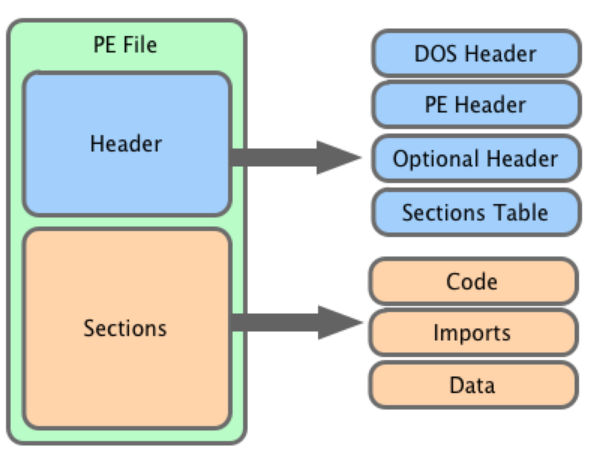
\includegraphics[scale=0.4]{img/FormatPE.png}
	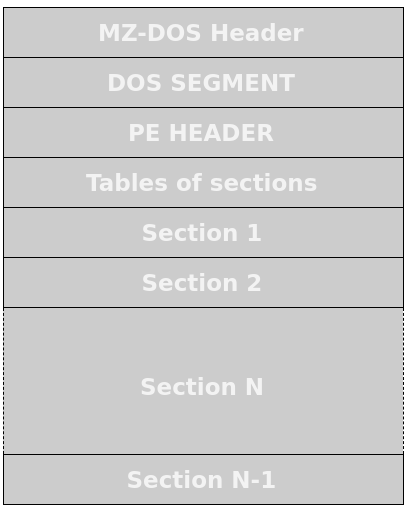
\includegraphics[scale=0.4]{img/FormatPE2.png}
\end{center}
\newpage
Un fichier standard PE contient généralement: 
\begin{itemize}[label=\textbullet]
	\item Une section .text (section de code)
	\item Une ou plusieurs sections de données (.data, .rdata ou .bss)
	\item Des tables de relocation généralement stockées dans la section .reloc
\end{itemize}

Une autre partie où l'on trouve les sections. Les sections sont en fait des sortes de répertoires dans lesquels sont regroupées des données ayant la même fonctionnalité, du code ou des ressources par exemple, sous un même attribut, qui peut être en lecture seule et écriture par exemple. Il faut donc bien voir ce système de sections qui est présent tout le reste du fichier. Ces sections contiennent le code, quelques informations sur le chargement en mémoire du fichier ou encore des informations de débogage. 

\chapter{Le Fuzzy hashing}
Il s’agit d’un outil dit de fuzzy hashing ceci signifie qu’une valeur de hash qui essaye de détecter le niveau de similarité entre deux fichiers au niveau binaire. Ce type de hash est différent d’un hash cryptographique tel que SHA1. Un hash cryptographique standard permet de répondre à la question “ c’est deux fichiers sont-ils identique ?” Un fuzzy hash aussi appelé similarity hash lui est utile pour répondre  à la question “une partie de ce fichier est-elle là même que ce second ?”
Les deux grands algorithmes de fuzzy hashing utilisé pour la classification de malware sont :
\begin{itemize}[label=\textbullet]
	\item \textbf{ssdeep : }
	\item \textbf{machocke : } Il s’agit d’un algorithme de fuzzy hashing basé sur le CFG
\end{itemize}

Il peut donc être intéressant d’utiliser ce hash comme feature. Nous n'avons malheureusement pas eu le temps de tester cette possibilité.
\chapter{Les différents type de ML}
\section{Supervisé}
\section{Non Supervisé}
\section{Les algorithmes}
\subsection{Classification}
La classification est une technique de machine learning supervisée qui est habituellement divisée en deux phases: La première phase consiste à former un classificateur en utilisant un algorithme de classification sur la base d’échantillon labellisé
\subsection{Clustering}
Le clustering est une technique de machine learning non supervisé elle permet de regrouper des données utilisant des similarités entre deux fichiers. Ceci signifie que des fichiers dans un  même cluster ( famille) sont très similaire les un des autres.
\subsubsection{KMeans}
Kmeans est l’un des algorithmes de clustering les plus populaire. Cette algorithme a pour objectif de partitionner n échantillons différents dans k clusters dans lequel chaque échantillons du même 


L'algorithme regroupe les données en essayant de séparer les échantillons dans n groupes de variance ég

Cet algorithme est bien adapté au grand nombre d’échantillons et au travers d’un large éventail de domaines très différents.
L'algorithme k-means divise un ensemble de N échantillons(samples) X en K cluster disjoints C, chacun décrit par la moyenne des échantillons dans le cluster. Les moyens sont communément appelés le cluster "centroïdes"; Remarque
qu'ils ne sont pas, en général, des points de X, bien qu'ils vivent dans le même espace. Le K-means
l'algorithme vise à choisir des centroïdes qui minimisent l'inertie, ou la somme intra-cluster du carré
critère.
\subsubsection{DBSCAN}

\subsubsection{Fuzzy-C Means}
Le fuzzy clustering (également appelée soft clustering) est une forme de clustering dans laquelle chaque point de données peut appartenir à plusieurs clusters. L'un des algorithmes de fuzzy clustering les plus utilisés est l'algorithme FCM (Fuzzy C-means Clustering).



\subsection{Analyse d'association}
\subsubsection{Méthode de Louvain}
C’est un algorithme hiérarchique proposé dans Blondel et al. (2008). L’algorithme itère sur deux étapes : 
1) Il cherche les petites communautés en optimisant la modularité de Newman et Girvan (2004) d’une manière locale.
 2) Il fusionne les nœuds de la même communautés et construit un nouveau réseau dont les nœuds sont les communautés. La partition qui a le maximum de modularité est retenue






















\part{Clustering & Malware}
\chapter{Etat de l'art}
Les progrès réalisés dans le domaine ces dernières année ont connu une croissance rapide généralement l’ensembles de données qui ont contribué à ces progrès sont accessible publiquement ( papier de recherche…), la présence de l’ensembles de ces données de référence publics et opensource nous permet de  suivre les progrès réalisés sur le terrain. Cependant, bien que les données ne manquent pas pour de nombreuses applications de machine learning les chercheurs en sécurité sont confrontés au problème inverse, les  jeux de données de référence on tendance à manquer. Ceci peut s’expliquer en partie en raison de la présence d'informations personnelles identifiables ou encore d'informations sensibles sur l'infrastructure réseau ou de propriété intellectuelle privée.

Le tableau n’a pas pour objectif d’être exhaustif  mais permet de comparer les jeux de données généralement utilisé dans les différentes recherche académique


\chapter{Implémentation}

\section{Introduction}
\begin{center}
	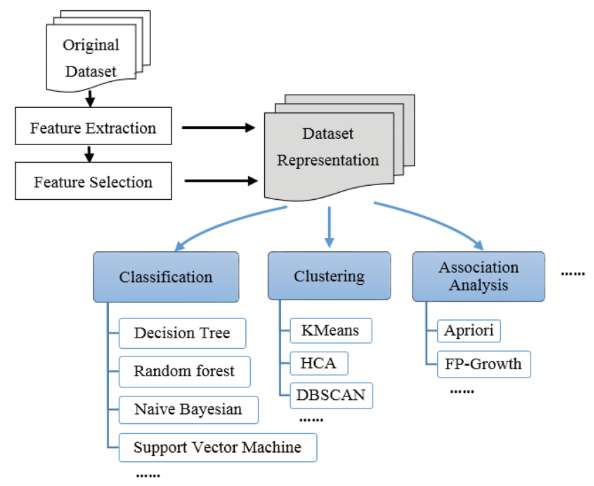
\includegraphics[scale=0.6]{img/Workflow.png}
\end{center}

Ci-dessus se trouve le déroulement classique de la création d’un modèle de machine learning.
L’un des gros problèmes et de trouver un jeu de données correcte et exploitable.
Une fois le jeu de données, il faut en extraire des éléments discriminant (réalisé par un expert sécurité). Des tests sont ensuite effectués afin de déterminer quelles sont les éléments discriminant qui permettent une meilleure détection.
\newpage

\section{Sélections des attributs}
L’étape d’extraction d’attributs est quant à elle spécifique à chaque problème de détection.

Dans le format PE, nous pouvons déjà isoler plusieurs informations intéressantes qui nous permettront de faire la différence entre un programme légitime et un malware. 

\textbf{Sections} : le nom, la taille, l'entropie, les caractéristiques.\newline
\textbf{Imports}: le nombre de modules, le nombre de symboles, les fonctions\newline
\textbf{Exports}: le nombre de modules, le nombre de symboles, les fonctions, la taille du fichier

Il est nécessaire de définir les attributs à extraire pour représenter les instances sous forme de vecteurs numériques :
\begin{itemize}[label=\textbullet]
	\item Les nombre de sections
	\item Les noms des sections
	\item L’entropie des sections
	\item Les DLL importées
	\item Les fonctions importées
	\item La distribution du jeu d’instruction x86
\end{itemize}


\section{Format des données - Extraction des features}
Afin de construire notre modèle de détection via du machine learning, il est nécessaire de récolter des données d'apprentissage. Il faut donc construire un dataset.

Pour constituer notre dataset qui servira par la suite à l’entrainement de notre algorithme de machine learning, nous allons essayer de générer  une collection de fichier au format JSON.
Dans ces fichiers chaque ligne contiendra un objet JSON. Nous avons tenté de définir une structure permettant de regrouper suffisamment d’informations.


Chacun de ces objets inclus les types de données suivant :

Il y a quelques grands principes à respecter lors de la construction du jeu d’apprentissage. Tout d’abord, il doit comporter un nombre suffisant d’instances pour que le modèle de détection soit capable de généraliser correctement les comportements bénin et malveillant.


Exemple de fichier JSON généré pour un fichier :
\lstset{
    string=[s]{"}{"},
    stringstyle=\color{blue},
    comment=[l]{:},
    commentstyle=\color{black},
}


\begin{lstlisting}

{
	"size": 106496,
	"path": "/home/light/Documents/Cours_CDSI/ML/dataset/theZoo/malwares/Binaries/VolatileCedar.Explosion/VolatileCedar.Explosion/0008065861f5b09195e51add72dacd3c4bbce6444711320ad349c7dab5bb97fb",
	"name": "0008065861f5b09195e51add72dacd3c4bbce6444711320ad349c7dab5bb97fb",
	"appeared": "2017-01",
	"label": "-1",
	"hashes": {
		"md5": "d2074d6273f41c34e8ba370aa9af46ad",
		"sha1": "5074ec3ca672f74ea05a7b5f0f52339fbf440f9b",
		"sha256": "0008065861f5b09195e51add72dacd3c4bbce6444711320ad349c7dab5bb97fb"
	},
	"nb_sections": 6,
	"nb_exported_fonctions": 7,
	"nb_imported_fonctions": 95,
	"exported_fonctions": ["CON", "Fdown", "Fdown2", "InetReadF", "_Comp@84", "_PathProcess@4", "_registerapp@8"],
	"imported_fonctions": ["InternetOpenA", "DeleteUrlCacheEntry", "InternetCloseHandle", "InternetOpenUrlA", "InternetReadFile", "CloseHandle", "GetCurrentProcessId", "GetModuleFileNameA", "GetModuleHandleA", "Sleep", "Module32First", "Process32Next", "Process32First", "CreateToolhelp32Snapshot", "InterlockedDecrement", "InterlockedIncrement", "CreateFileA", "WinExec", "TlsSetValue", "GetLocaleInfoW", "HeapSize", "HeapFree", "ExitProcess", "RtlUnwind", "RaiseException", "GetCurrentThreadId", "GetCommandLineA", "GetVersionExA", "HeapDestroy", "HeapCreate", "VirtualFree", "DeleteCriticalSection", "LeaveCriticalSection", "EnterCriticalSection", "HeapAlloc", "VirtualAlloc", "HeapReAlloc", "IsBadWritePtr", "QueryPerformanceCounter", "GetTickCount", "GetSystemTimeAsFileTime", "TlsAlloc", "SetLastError", "GetLastError", "TlsFree", "SetEndOfFile", "TlsGetValue", "GetProcAddress", "SetUnhandledExceptionFilter", "LCMapStringA", "WideCharToMultiByte", "MultiByteToWideChar", "LCMapStringW", "WriteFile", "FlushFileBuffers", "SetFilePointer", "TerminateProcess", "GetCurrentProcess", "SetHandleCount", "GetStdHandle", "GetFileType", "GetStartupInfoA", "FreeEnvironmentStringsA", "GetEnvironmentStrings", "FreeEnvironmentStringsW", "GetEnvironmentStringsW", "UnhandledExceptionFilter", "InitializeCriticalSection", "InterlockedExchange", "VirtualQuery", "LoadLibraryA", "IsBadReadPtr", "IsBadCodePtr", "GetACP", "GetOEMCP", "GetCPInfo", "GetLocaleInfoA", "VirtualProtect", "GetSystemInfo", "GetStringTypeA", "GetStringTypeW", "GetUserDefaultLCID", "EnumSystemLocalesA", "IsValidLocale", "IsValidCodePage", "SetStdHandle", "ReadFile", "RegCreateKeyA", "RegSetValueExA", "RegOpenKeyExA", "RegDeleteValueA", "RegCloseKey", "RegCreateKeyExA", "connect", "URLDownloadToFileA"],
	"imported_libraries": ["WININET.dll", "KERNEL32.dll", "ADVAPI32.dll", "WS2_32.dll", "urlmon.dll"],
	"general": {
		"vsize": 118784,
		"has_debug": 1,
		"exports": 7,
		"imports": 95,
		"has_relocations": 1,
		"has_resources": 1,
		"has_signature": 0,
		"has_tls": 0,
		"symbols": 0,
		"entrypoint": "0x100055dc"
	},
	"header": {
		"coff": {
			"timestamp": 1383637370,
			"machine": "I386",
			"characteristics": ["CHARA_32BIT_MACHINE", "DLL", "EXECUTABLE_IMAGE", "LINE_NUMS_STRIPPED", "LOCAL_SYMS_STRIPPED"]
		},
		"optional": {
			"subsystem": "WINDOWS_GUI",
			"dll_characteristics": [],
			"magic": "PE32",
			"major_image_version": 0,
			"minor_image_version": 0,
			"major_linker_version": 7,
			"minor_linker_version": 10,
			"major_operating_system_version": 4,
			"minor_operating_system_version": 0,
			"major_subsystem_version": 4,
			"minor_subsystem_version": 0,
			"sizeof_code": 65536,
			"sizeof_headers": 4096,
			"sizeof_heap_commit": 4096
		}
	},
	"sections": [{
		"name": ".text",
		"characteristics": 1610612768,
		"vsize": "0xf2eb",
		"size": "0x10000",
		"vaddres": "0x1000",
		"entropy": 6.625413677157515
	}, {
		"name": ".rdata",
		"characteristics": 1073741888,
		"vsize": "0x3a3b",
		"size": "0x4000",
		"vaddres": "0x11000",
		"entropy": 5.043471612579925
	}, {
		"name": ".data",
		"characteristics": 3221225536,
		"vsize": "0x3358",
		"size": "0x1000",
		"vaddres": "0x15000",
		"entropy": 2.7813728969479183
	}, {
		"name": ".SHARDAT",
		"characteristics": 3489660992,
		"vsize": "0x8",
		"size": "0x1000",
		"vaddres": "0x19000",
		"entropy": -0.0
	}, {
		"name": ".rsrc",
		"characteristics": 1073741888,
		"vsize": "0x368",
		"size": "0x1000",
		"vaddres": "0x1a000",
		"entropy": 3.2077393530680016
	}, {
		"name": ".reloc",
		"characteristics": 1107296320,
		"vsize": "0x1630",
		"size": "0x2000",
		"vaddres": "0x1b000",
		"entropy": 5.857932346902008
	}]
}
\end{lstlisting}

\section{Choix technologiques}
Afin d’implémenter notre algorithme de machine learning et d’effectuer des testes, nous avons parcours l’ensemble des technologies disponible aujourd’hui voici celles que nous avons retenue :

\subsection{Redis}
REmote DIctionary Server qui peut être traduit par « serveur de dictionnaire distant » et jeu de mot avec Redistribute1) est un système de gestion de base de données clef-valeur scalable, très hautes performances, écrit en C ANSI et distribué sous licence BSD. Il fait partie de la mouvance NoSQL et vise à fournir les performances les plus élevées possibles. 

Nous aurions pu utiliser d'autres base de données noSQL tel que Spark, MongoDB, très utilisé dans le BigData.

\subsection{SciPy}
SciPy est un projet visant à unifier et fédérer un ensemble de bibliothèques Python à usage scientifique. Scipy utilise les tableaux et matrices du module NumPy.
Cette distribution de modules est destinée à être utilisée avec le langage interprété Python.

pandas
Numpy

\subsection{Scikit-learn}
Nous avons utilisé Scikit-learn est une bibliothèque libre Python dédiée à l'apprentissage automatique. Il existe beaucoup d’autre framework python tel que tensorflow ou encore pytorch. Suite à nos recherches Scikit learn semblait être le mieu documenté et posséder une très grande communauté.

\subsection{LIEF : Library to Instrument Executable Formats}
Pour notre projet comme de nombreux autre nous avons besoin d'analyser les formats exécutables la majorité des projets  ré-implémentent généralement leur propre analyseur de fichier exécutable. Dans les délais impartie étant données que nous ne maîtrisons pas suffisamment bien le format PE. Il n’est pas envisageable de développer de zéro un parser de fichier.
De plus, ces parseurs de fichier sont généralement liés à un langage de programmation particulier.

LIEF : Library to Instrument Executable Formats est un projet initié par QuarksLab qui a pour objectif d’offrir une librairie cross platform qui peut parser et modifier les différents format de fichier ELF, PE, MachO. Cette librairie offre une couche d’abstraction.
Le projet fournit une API Python C/C++

\begin{center}
	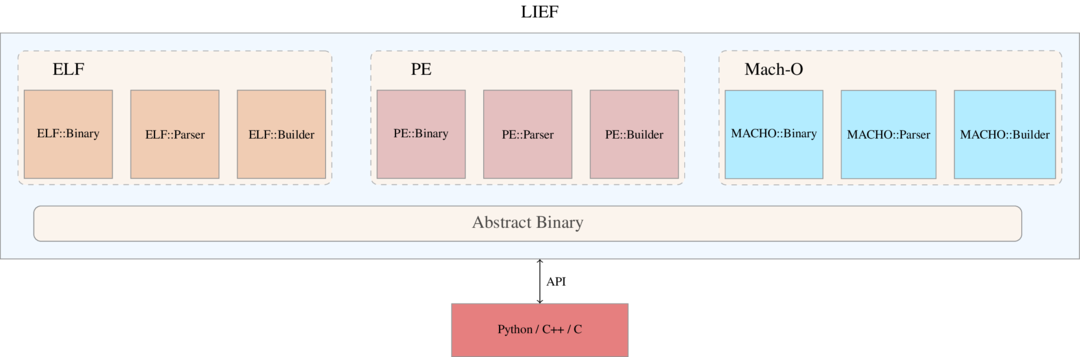
\includegraphics[scale=0.475]{img/archi.png}
\end{center}

\subsection{Capstone engine}
Il s'agit d'un framework de multiplateforme et multiarchitecture qui permet le désassemblage de fichier.

\subsection{Radare2} est un framework de reverse engineering, il embarque le moteur capstone pour le désassemblage. Radare2 est instrumentale en python à travers r2pipe.

\chapter{Code - Python}

Nous avons utilisé le repository TheZOO comme dataset dans un premier temps il contient des malwares et est disponible sur github. 


Notre projet est composé de divers scripts:
Vous pouvez le retrouver ici : \newline
"https://github.com/lightoyou/Malware\_Clustering\_ML"

Nous allons les parcourir ensemble afin de comprendre leurs objectifs.

\begin{itemize}[label=\textbullet]
	\item Le premier script est \textbf{PEtoJSON.py}
	Ce script permet à partir d’un jeu de données binaire grâce à la librairie LIEF d’extraire les informations sur les fichiers de façon statique. Le script prend en entré un répertoire ou il va naviguer de façon récursive afin de passer sur chaque fichier.
A l’issue de la procédure un fichier au format JSON portant le sha256 du fichier est créer dans le répertoire jsonfiles.
Des améliorations sont encore possible (extraction de strings….). Cependant les informations essentiel sont actuellement présente.
Exemple présentez précédemment.


\item Le second script est \textbf{extract\_features.py} \newline
Ce script permet de parcourir l’intégralité des fichiers json, d’en isoler un vecteur de features : 
features = ["size\_of\_file","number\_of\_sections","median\_of\_entropy","nb\_of\_imports","number of exports"]
\newline Un second vecteur de features pourraient être mis en place afin de comparer les résultats cependant par manques de temps nous n’avons pas eu le temps de tester.

Nous utilisons un serveur redis pour mettre en cache et améliorer les performances du traitement. La bibliothèque numpy est utilisé afin de sauvegarder ce vecteur de feature sous forme de fichier .npy.

\item Les scripts est \textbf{learnKmeans.py} et \textbf{learnDBSCAN.py}
\subitem Ce LeanKmeans  utilise l'algorithme Kmeans via la bibliothèque sikitlearn. 

KMeans = KMeans(n\_clusters=90,n\_jobs=8,precompute\_distances=False)
Nous définissons que nous définissons le nombres de clusters (de catégories de malwares) ainsi que le nombre de jobs ( pour effectuer le calcule).



\subitem  Ce  \textbf{LeanDBSCAN}  utilise l'algorithme \textbf{DBSCAN} via la bibliothèque sikitlearn.


\item Le script \textbf{parse\_vt\_report.py}
Nous pouvons continuer le processus sur un jeu de données plus conséquent. Nous avons commencé le travaille sur les fichiers présent sur VirusShare.
Il s’agit d’un gros dataset de fichier malveillant.
Nous avons au cours de nos recherches récupérer des fichiers json contenant les rapports VirusTotal de l’intégralité des malwares de virushare. (utilisation de l’API par un groupe de recherche).
Ces rapports permettent de labéliser l’intégralité dataset aux travers le résultats de différents antivirus.
Un gros travaille est à faire afin de normaliser ce jeu de données. 
Nous avons développé un script parse\_vt\_report.py qui permet de faire une prédiction sur la catégorie du bénin (ransomware, virus, ver...).
Nous aurions voulus réaliser notre propre dataset afin d’effectuer à la fois de la classification et du clustering. Cependant cette tâche est compliqué et nécessite beaucoup de travaille nous ne sommes pas parvenu à cette étape. Nous aurions aimé continuer.


Globalement les fichiers manques de documentation et de commentaires. Nous en sommes conscient.

\end{itemize}




\chapter{Nos résultats}
Dans cette partie nous allons essayé de choisir un type de modèle de classification adapté aux contraintes opérationnelles et de comparer les résultats de détection obtenues sur différents algorithmes.

\section{K-Means}

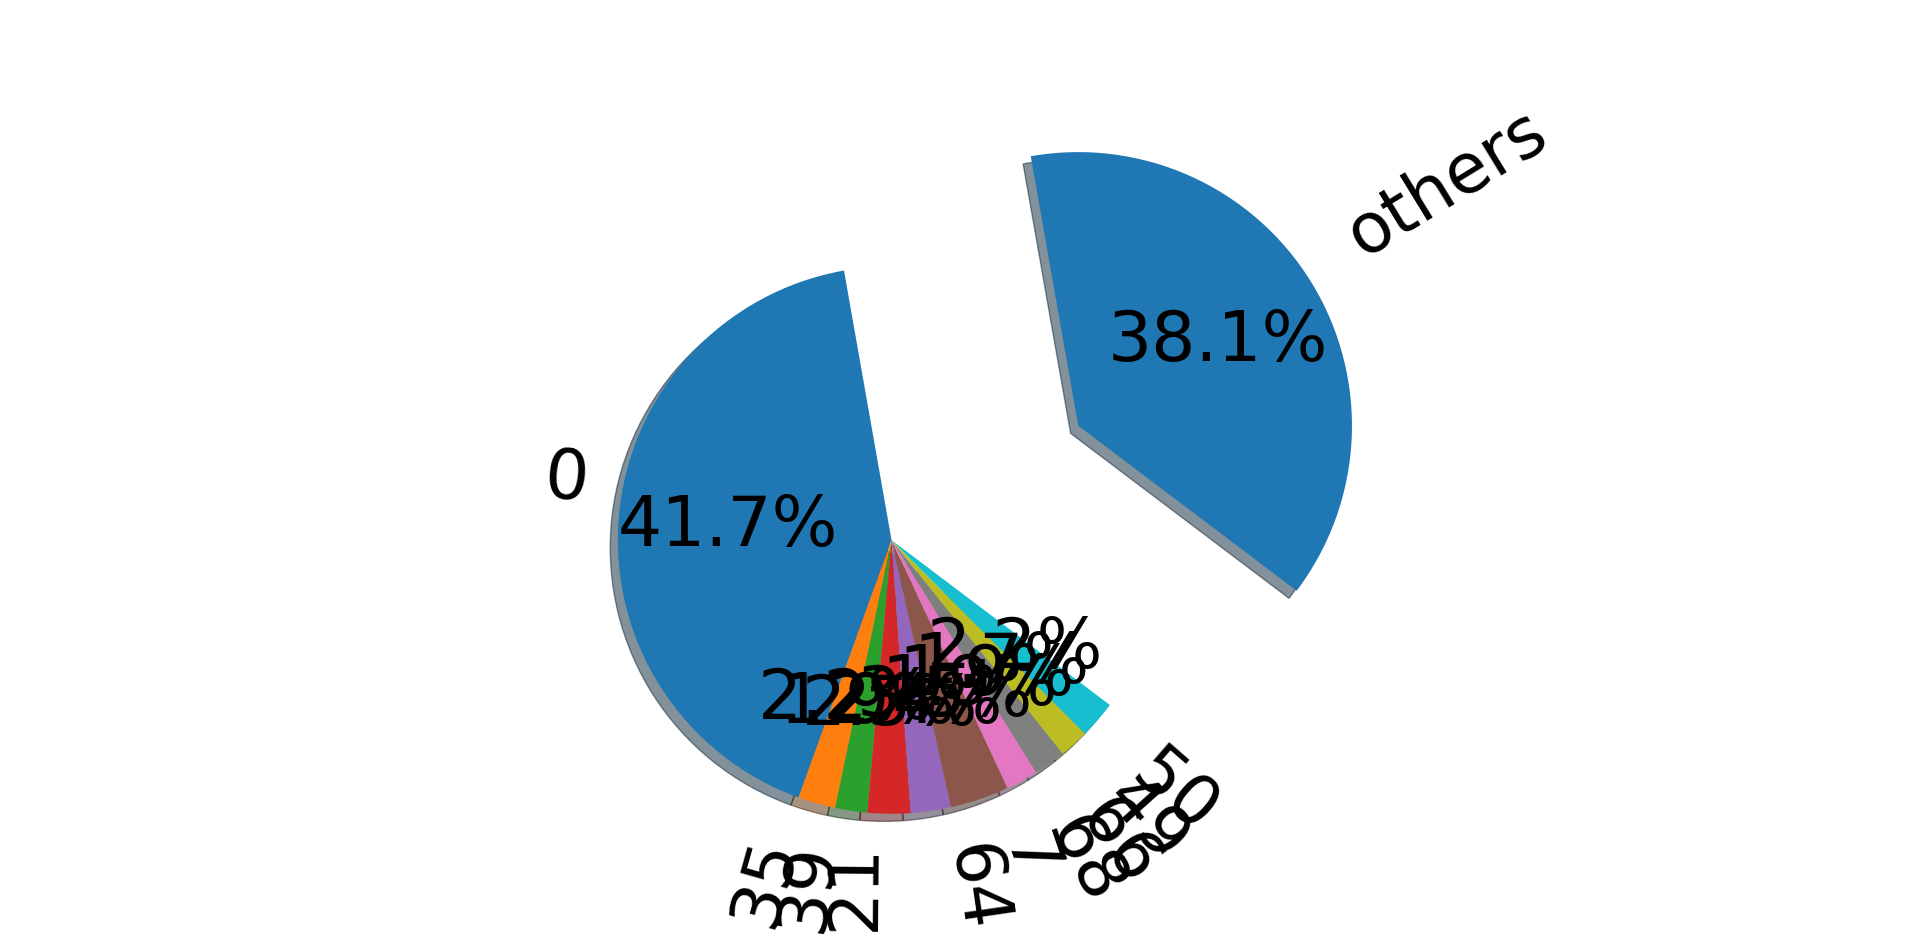
\includegraphics[scale=0.4]{img/results/Kmeans.png}
Ce graphique présente la distribution des malwares du dataset TheZoo que nous avons utilisé.
Nous pouvons noter deux grandes catégories :

Counter({b'EquationGroup': 261, b'EquationGroup.Fanny': 1, b'Backdoor.MSIL.Tyupkin': 1, b'Ransomware.Locky': 1})


Nous remarquons qu'un gros cluster de malware EquationGroup est majoritaire. Notre jeu n’est pas très homogène et n’est pas représentatif des fichiers pouvant être trouvé dans la nature.

Ces premiers résultats sont intéressant mais pas totalement efficient.
Quand on regarde la phase de normalisation du vecteur, la taille joue un rôle important. Cette feature a tendance à écraser les autres valeurs. Il pourrait donc être intéressant de normaliser en utilisant la valeur max de chaque features. 
La phase de normalisation est très importante.


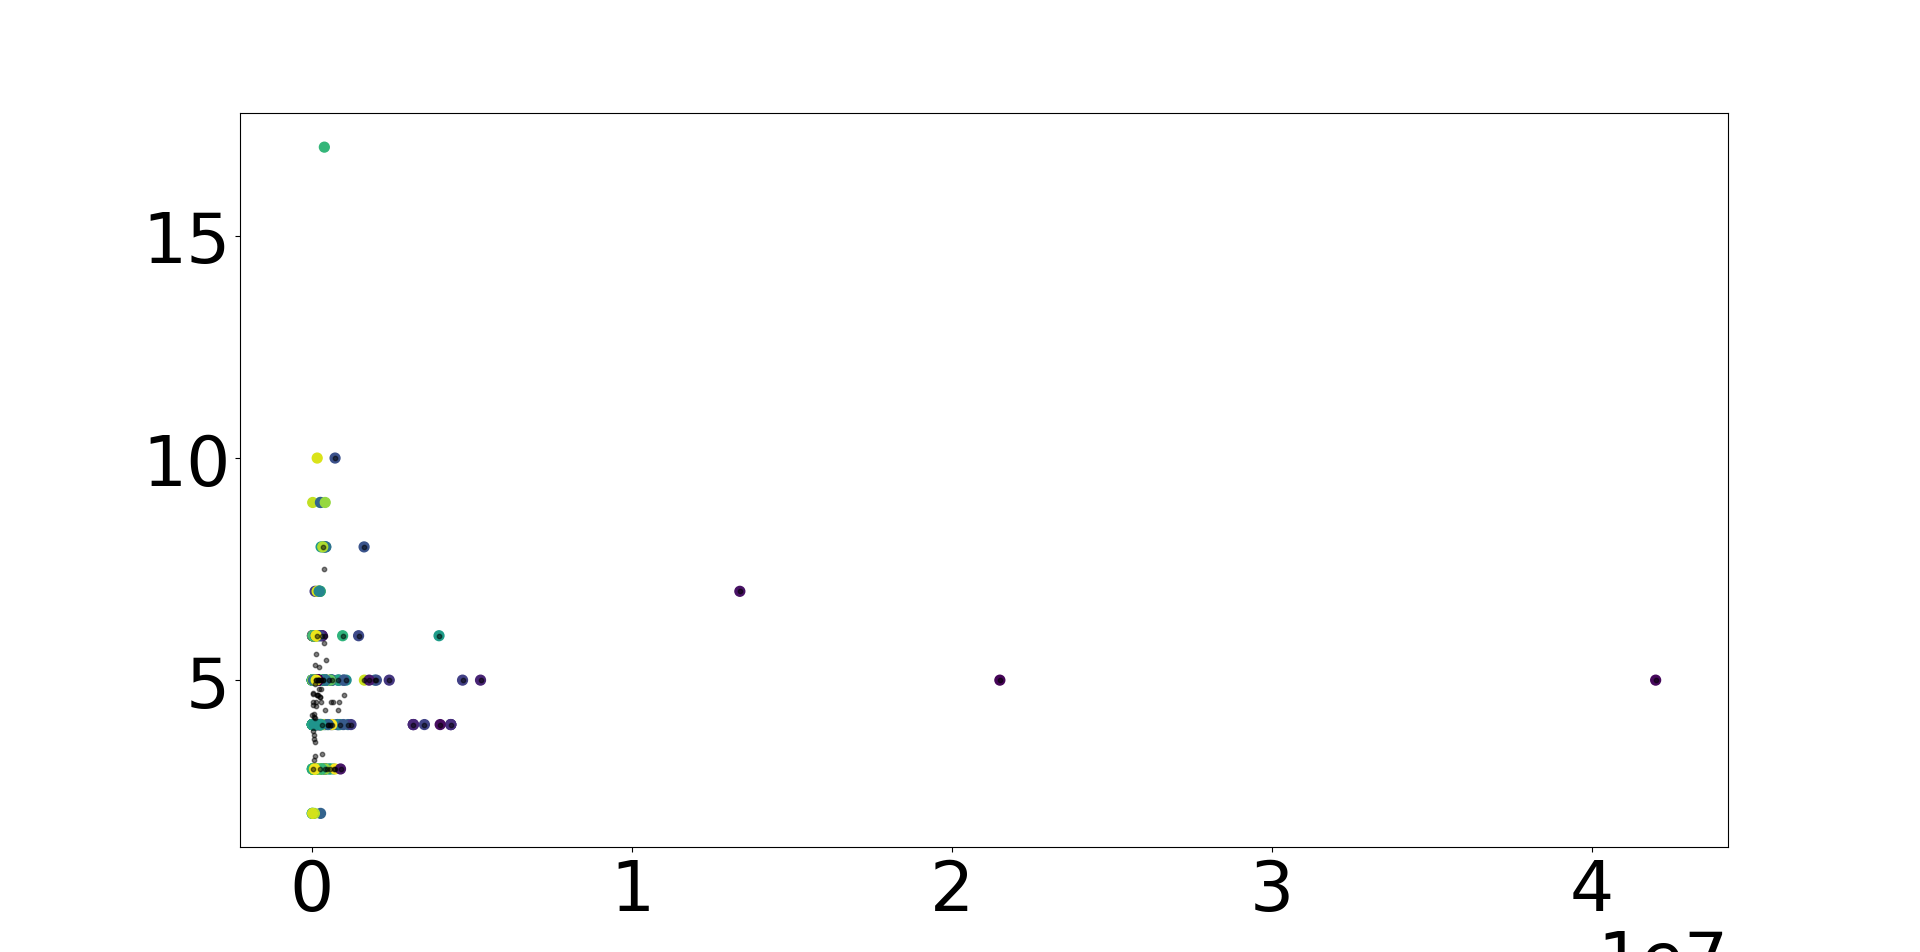
\includegraphics[scale=0.4]{img/results/dataset.png}
La figure ci-dessus permet de représenter la répartition du jeu de donnée par rapport au centroide.

\section{DBSCAN}
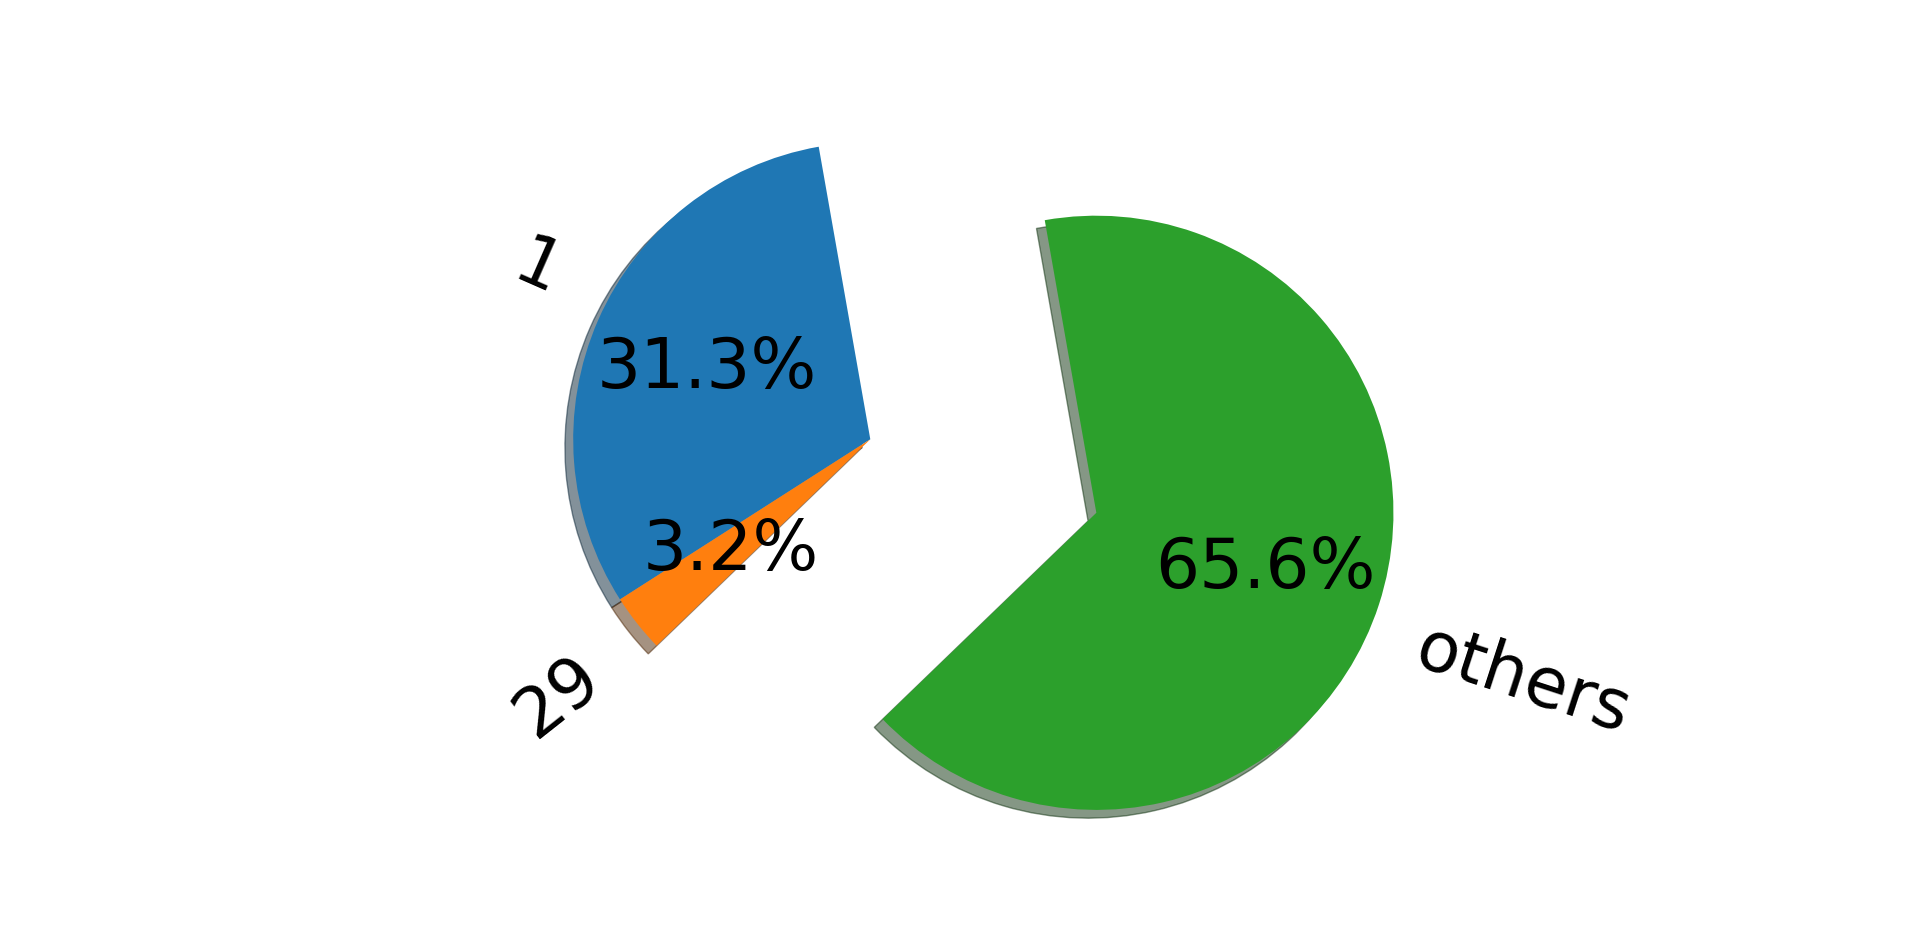
\includegraphics[scale=0.4]{img/results/dbscan.png}

\textbf{Catégorie 1}

[(b'003315b0aea2fcb9f77d29223dd8947d0e6792b3a0227e054be8eb2a11f443d9', b'EquationGroup.Fanny'), (b'022224bfad26bab87cf5f4b17981a4224ef8fa6919520b3bc2946234efda1e11', b'EquationGroup'), (b'037bdc95919b1d3d65af6202e8c9c9ca3caba7a863e4e39162b93fa032881feb', b'EquationGroup'), (b'045f0ecae2362355f06d4fc8fa97e577daad1e01e6f0c0523b5b0f9e15306c74', b'EquationGroup'), (b'083c64c404ac1ea6df1a4cb6eafa91ef90b7abacc54547cf008cd74e77195746', b'EquationGroup'), b227be1967cd3bf0171bc36f18eb3616265cf62f8c4631fd98121ac48af2', b'Equ
\newline
\textbf{Catégorie 29}
(b'12e8654f7ce06a2bfad58884cb44f745db618feae49dc17419857b491fbdca0c', b'EquationGroup'), (b'140405af287d7d44ae06fdd169e8c3ee9033a7b3a43890a72114efb16b5a17cc', b'EquationGroup'), (b'2e48d5bd7f6aba93f5a8af37defcd1b0cb6375335eeeceb3dc060ab6f7dcd2d7', b'EquationGroup'), (b'3b96240880b2fc4d9d05e85e4e47e5cf1f431c551b77a88ee9f21eacd4c5d157', b'EquationGroup'), (b'427c68a1c5ecb37a15af1cdfbaf9cc35448a4c148514f7b6c06a7ac266f76068', b'EquationGroup'), 

Ces premiers résultats sont intéressant mais pas totalement efficient.
Quand on regarde la phase de normalisation du vecteur, la taille joue un rôle important. Cette feature a tendance à écraser les autres valeurs. Il pourrait donc être intéressant de normaliser en utilisant la valeur max de chaque features. 
La phase de normalisation est très importante.



Des testes approfondies sur le d’autres algorithme tel que Dbscan sont nécessaire. D’autres vecteurs de de features doivent être testé afin de comparer les résultats. L’intégration par exemple de vecteur tel que des chaînes de caractères ( regex sur des registres, des urls…). Nous pouvons nous baser sur des travaux tel que les n-gram.
Nous devons exploiter les résultats actuels afin de mieux comprendre et identifier les caractéristiques les plus pertinentes pour la classification.

Nos testes sur un petit jeu de données nous ont permis de comprendre le fonctionnement de base du machine learning.



\chapter{Conclusion}
À travers cet article nous pouvons en conclure que le machine learning ce n’est pas magique, un gros travail de featuring est nécessaire. Un bon jeu de données de départ est aussi très important.
Le multi-architecture et l’extension vers d’autres type de virus que ceux ciblant Windows est facilement envisageable grâce à la library LIEF.
Le machine learning est très utile pour faire un premier filtre afin de catégoriser un gros jeu de données comparé à des algorithmes de fuzzy hashing.






L’utilisation de LightGBM




L’état actuel de nos travaux nous permet de conclure que cette méthode est pertinente et efficace car les résultats obtenus sont déjà très bons alors que de nombreuses pistes sont encore disponibles pour l’améliorer.
Nous avons uniquement implémenté une solution permettant de faire du clustering, nous aimerions par la suite nous tourner vers des algorithmes de classification.

\chapter{Glossaire}
\textbf{Machine Learning :} Retrouver des patterns dans un jeu de données afin de les regrouper.

\textbf{Classification :} Classer les données dans des catégories prédéfinies. Les algorithmes sont par exemple : decision Tree, Random forest ect.

\textbf{Clustering :} Regrouper les données dans un ensemble de catégories. Les algorithmes sont par exemple : KMEans, HCA, DBSCAN ect.

\textbf{Feature :} Caractéristique d’un objet utile pour l'algorithme (les patterns potentiels).

\textbf{Vector of features :} Un tableau de features.

\textbf{Cluster :} Un groupe d’objets décidé par l'algorithme.

\textbf{Label :} Nom du cluster.

\textbf{CFG :} En informatique, un graphe de flot de contrôle (abrégé en GFC, Control Flow Graph ou CFG en anglais) est une représentation sous forme de graphe de tous les chemins qui peuvent être suivis par un programme durant son exécution.

\textbf{JSON :} JavaScript Object Notation (JSON) est un format de données textuelles dérivé de la notation des objets du langage JavaScript. Celui-ci permet de représenter de l’information structuré comme le permet XML par exemple.

\chapter{Bibliographie}
\textbf{Schultz, et al., 2001 :} \url{http://128.59.14.66/sites/default/files/binaryeval-ieeesp01.pdf}

\textbf{Kolter and Maloof, 2006 :} \url{http://www.jmlr.org/papers/volume7/kolter06a/kolter06a.pdf}

\textbf{Shafiq et al., 2009 :} \url{https://www.researchgate.net/profile/Fauzan_Mirza/publication/242084613_A_Framework_for_Efficient_Mining_of_Structural_Information_to_Detect_Zero-Day_Malicious_Portable_Executables/links/0c96052e191668c3d5000000.pdf}

\textbf{Raman, 2012 :} \url{http://2012.infosecsouthwest.com/files/speaker_materials/ISSW2012_Selecting_Features_to_Classify_Malware.pdf}

\textbf{Saxe and Berlin, 2015 :} \url{https://arxiv.org/pdf/1508.03096.pdf}

\end{document}